 
\section{Scientific Objectives}

The scientific outcome of this instrument proposal is in accordance
with ESA \ac{SciRD}\cite{yellowbook} and addresses many of the scientific
investigations proposed in the ESA JUICE Assessment Study Report\cite{yellowbook}.


\subsection{Introduction \label{sub:Introduction-science}}

The GIPER instrument is part of the JUICE mission which will investigate
the Jupiter system with special interest in the moons Ganymede and
Europa. So far most of the information about Jupiter and its satellites
originates from the flybys of Voyager 1 and 2 in the end of the 1970ies
and to the most extend from the Galileo mission started in 1989 and
ended in 2003. The objective of the Galileo mission was to investigate
the Jupiter system and especially the weather on Jupiter. Therefore
most instruments were focusing on imaging and the measuring of particles
and fields. The JUICE mission will focus on getting an insight on
the Galilean moons of Jupiter, especially Ganymede and Europa. The
moons consist mainly of solid constituents, therefore a different
set of instrument is needed for thorough investigation. The introduced
GIPER instrument focuses on the moon Ganymede, but as also Europa
and to some extend Callisto have also a surface consisting mostly
of ice, thus applications for these moons are available too.

Ganymede is the largest moon in the Jovian System and one of the four
Galilean moon. It was discovered in 1610 by Galileo Galilei. With
a mean radius of 2634~km Ganymede is the largest moon in the Solar
System and even larger than the planet Mercury. It travels around
Jupiter in an orbit with a semi-major axis of $1070400$~km and an
eccentricity of 0.00013. It is therefore the third of the Galilean
moons\cite{pater2010planetary}. 

It is believed that Ganymede consists mainly of 3 layers which are
fully differentiated. The core consists of a hot iron alloy which
is responsible for generating the intrinsic magnetic field. The second
layer is made of heavier rocky material and the third layer consists
mainly of water ice. The icy surface is expected to be around 800~km
thick. On the boundary between the icy and the rocky layer large oceans
of liquid water may be present\cite{bagenal2007jupiter}.


\subsubsection{The surface composition of Ganymede}

The main understanding of the surface composition and the underlying
processes of forming of Ganymede originates from the Galileo mission
and partly from the flybys of Voyager 1 and 2. A true color image
of the Ganymede surface taken from the Galileo orbiter is show in
figure \ref{fig:Ganymed-true-color}. It consists mainly of water
ice and is basically separated into regions with a low albedo, often
referred to as dark terrain, which covers about 34~\% of the surface
and regions of high albedo, named bright terrain respectively, which
covers 66~\%\cite{bagenal2007jupiter}. The boundaries between dark
and bright terrain are mostly sharp and distinct. The dark terrain
is covered with a much higher amount of impact craters. It is therefore
believed to be much older than the bright terrain which could be as
young as 1 billion years\cite{Showman2004}. Stereo images suggests
that the dark furrow terrain is generally higher than the grooved
bright terrain. This leads to the idea that bright terrain has probably
formed by tectonic processes of the (former) dark terrain together
with transport processes of snow or water to the surface like cryo-volcanism
(see also section \ref{sub:volcanism}) thereby smoothing the surface.
Impact craters of meteoroids therefore show up as bright white spots
on the white terrain\cite{Schenk2001,Patterson2010,bagenal2007jupiter,Showman1997,Showman2004}. 

\begin{figure}
\begin{centering}
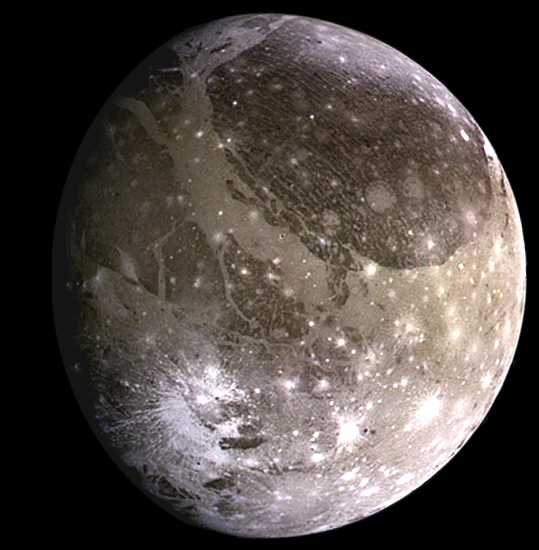
\includegraphics[width=0.7\textwidth]{Figures/Ganymede_true_color}
\par\end{centering}

\caption{True color image of Ganymede's surface taken by the Galileo spacecraft.\label{fig:Ganymed-true-color}}


\end{figure}



\subsubsection{Formation of the surface and sub-surface processes\label{sub:volcanism}}

The processes causing the formation of the bright terrain from the
ancient dark terrain are believed to be tectonics and cryo-volcanism
although they are still not fully understood and part of active discussions\cite{Showman2004,Schenk2001,Patterson2010}.
Most models need a heat source strong enough to (partly) melt sub-surface
layers. The current orbital parameters of Ganymede would not be sufficient
to produce enough heat by tidal forces, orbital calculations suggest
that Ganymede had a period where the eccentricity of its orbit reached
as high as 0.03\cite{Showman1997} which would cause enough tidal
heating to melt parts of the icy interior up to an extend where the
moon extends up to 1~\% causing major tectonic movements and the
formation of grabens\cite{Showman2004}. 

Another unknown problem is the transport of the then (partly) molten
ice or slush to the surface in order to fill graben. One proposition
is that icy ,,volcanoes`` ejected low-viscous liquid water which
then flooded the graben before freezing. So far no strong evidences
for this volcanism like ejection centers or downstream patterns on
the horsts have been found\cite{Patterson2010}. This may be because
the resolution of the images obtained by the Galileo and Voyager missions
do not have a high enough resolution, the areas for which high resolution
pictures are available do not have pronounced enough evidences or
there are just not existent\cite{Patterson2010,Schenk2001,Showman2004}.
Another problem is that water or slush have a higher density than
ice, thus if tidal heating would melt ice, the water or slush would
sink deeper instead of rising to the top.

An approach to solve this issue proposed by Showman and Mosqueira
would also explain why there is no ice on top on the horsts and the
lack of flooding tracks is that tectonics resurfaced the dark terrain
to contain horsts and grabens. These apply different pressure to the
underlying terrain. These pressure gradients could actually lead to
the circumstance that material with a negative buoyancy like water
or slush could move upwards but only below the grabens. When the graben
are filled with ice, the process automatically stops because the necessary
pressure imbalance from the terrain disappears hence no ice could
reach the high horsts\cite{Showman2004}. 

In figure \ref{fig:gradients} an example calculation for the gradients
due to terrain imbalance is presented. The terrain was modeled as
a sine wave with 30~km wavelength and an amplitude of 1~km (2~km
peak-to-peak) as shown in the top graphic of figure \ref{fig:gradients}.
\begin{figure}
\begin{centering}
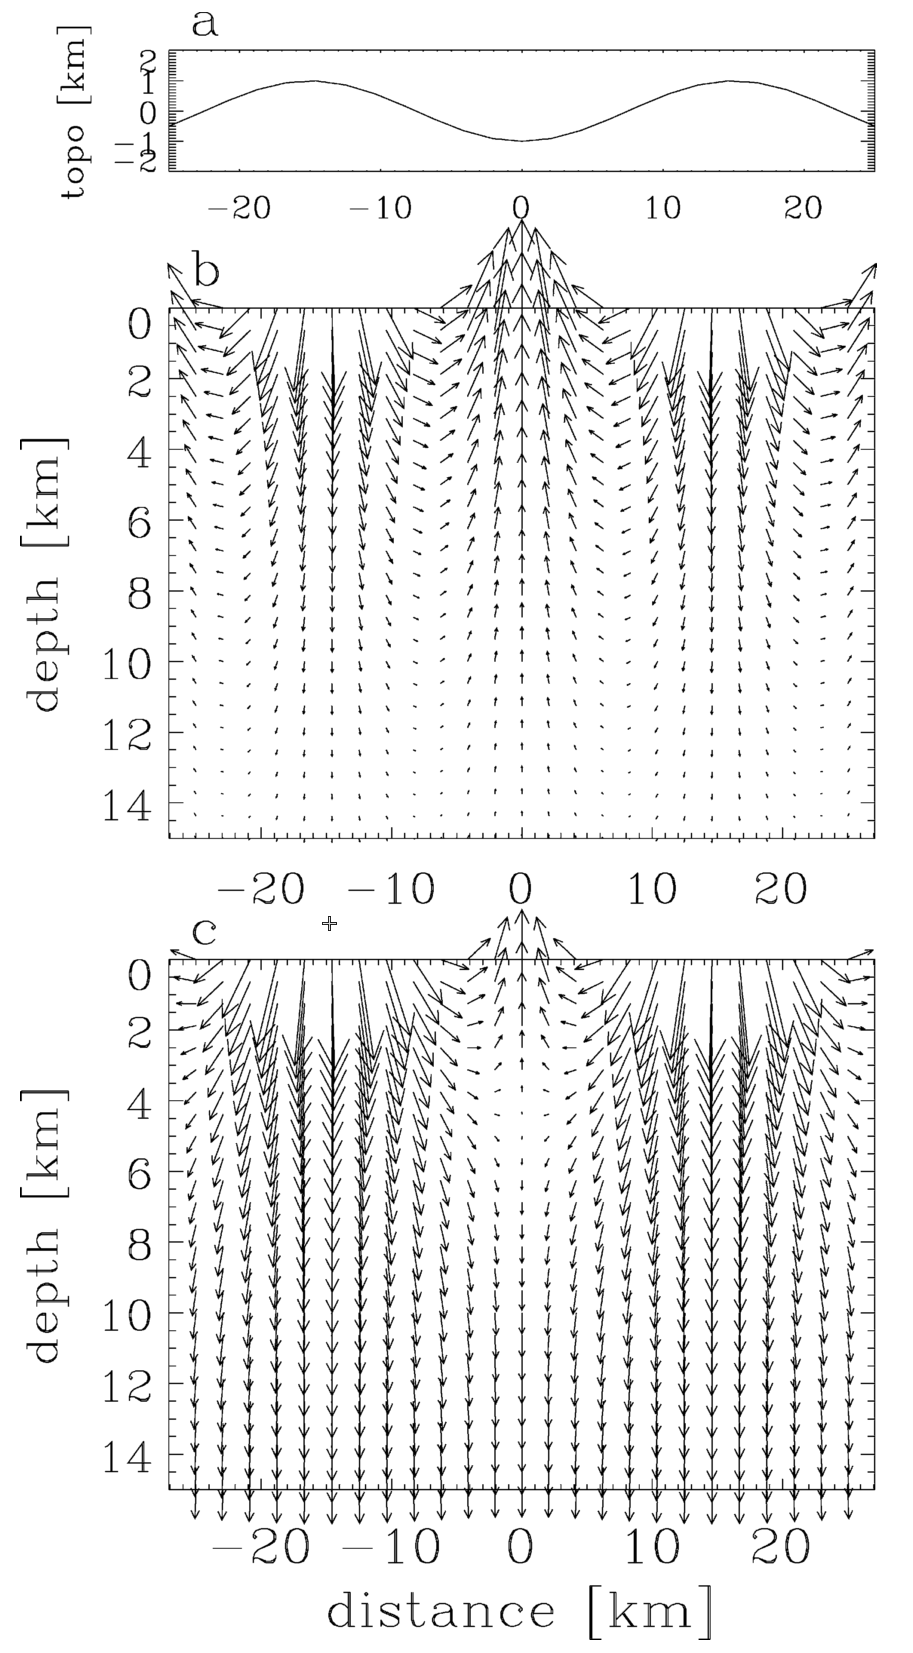
\includegraphics[width=0.7\textwidth]{Figures/gradients}
\par\end{centering}

\caption{Example calculation for \textbf{(a)} a sinusodial terrain with an
amplitude of 1~km and a wavelength of 30~km. The (b) pressure gradient
from the tectonic imbalance can compensate the negative byuoancy of
water in lower surface areas up to 5~km (c). Figure taken from \cite{Showman2004}\label{fig:gradients}}


\end{figure}
 The vector plot in the middle shows the resulting pressure gradients.
As can be seen underneath the graben they are directed upwards but
decrease exponentially with depth. The lower vector plot shows the
resulting gradients when considering water with a negative buoyancy.
As can be seen water could only move up to the surface when it is
created in a depth below 5~km. Further calculations performed by
Showman, Mosqueira et al. estimate that depth from where water or
slush can rise to the surface ranges from 5~km to 10~km. A possible
problem with this model may be that is would need at lease 1 million
years to transport enough water to the surface in order to fill grabens,
but the graben could relax gravitationally earlier and thus stop the
upward flow\cite{Showman2004}. 

In order to find the dominant processes for the resurfacing of Ganymede's
dark terrain it would be essential to acquire measurements from the
subsurface interior additionally to (new) surface pictures. Ganymede
can be seen as a prototype for an icy body. Therefore investigating
the tectonic processes of Ganymede and its surface evolution will
not only provide more information about the formation of Ganymede
but also of its siblings Europa and Callisto as well as icy bodies
in general \cite{bagenal2007jupiter}.


\subsection{Scientific Goals\label{sub:Scientific-Goals}}

Based on the short scientific introduction of Ganymede from section
\ref{sub:Introduction-science} the following scientific goals can
be identified:
\begin{itemize}
\item Map the interior below the surface of Ganymede to get more insight
about different layers and their composition. 
\item Find evidences for the tectonic processes which created the horsts
and grabens of the grooved terrain
\item Find out how did the dark and bright terrain evolve over time.
\item Find evidences for or against different cryo-volcanism scenarios
\item Get a more detailed map of the surface terrain compared to stereoscopic
imaging
\item Possibility to find habitable zones 
\end{itemize}

\subsection{Scientific Performance Requirements}

In order to achieve the goals described in section \ref{sub:Scientific-Goals}
the instrument should be able to penetrate the surface to at least
5~km. Attenuation of radar waves in the lower MHz spectrum in ice
is quite small which is beneficial for a high penetration depth, but
although it is quite certain that the upper surface mainly consists
of water ice there might be significant amounts of rocky material
at some parts due to the many meteoroid impacts after the accretion
phase of Ganymede. Therefore an appropriate margin for the penetration
depths should be considered. 

The vertical resolution should be in the range of 10~m -- 35~m to
give the chance to resolve the position and offset of the identified
layers with high accuracy. A typical width for the groves of the terrain
is 10~km, thus the horizontal resolution should not exceed this value
in order to correlate different vertical layers to the surface terrain. 

As the goal is to create a map of the whole surface of Ganymede it
is expected that even after preprocessing and compression a large
amount of data will be collected. An appropriate downlink capacity
should be reserved for the mission.

